% Figure: All algorithms comparison (log-log scale)
\begin{figure}[t]
\centering
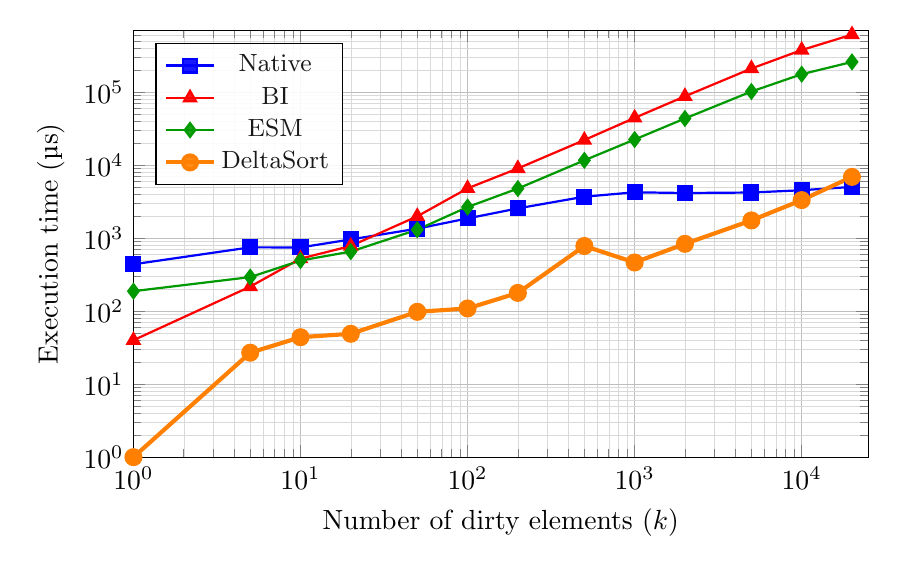
\begin{tikzpicture}
\begin{axis}[
    width=0.9\textwidth,
    height=7cm,
    xlabel={Number of dirty elements ($k$)},
    ylabel={Execution time (\textmu s)},
    xmode=log,
    ymode=log,
    log basis x=10,
    log basis y=10,
    xmin=1, xmax=25000,
    ymin=1, ymax=700000,
    legend pos=north west,
    legend style={font=\small, fill=white, fill opacity=0.9},
    grid=both,
    grid style={line width=0.1pt, draw=gray!30},
    major grid style={line width=0.2pt, draw=gray!50},
]

% Native sort
\addplot[color=blue, mark=square*, thick, mark size=2.5pt] coordinates {
    (1, 439) (5, 749) (10, 747) (20, 962) (50, 1350) (100, 1867) 
    (200, 2560) (500, 3703) (1000, 4253) (2000, 4158) 
    (5000, 4223) (10000, 4539) (20000, 5042)
};

% Binary Insertion
\addplot[color=red, mark=triangle*, thick, mark size=2.5pt] coordinates {
    (1, 40) (5, 217) (10, 525) (20, 782) (50, 1994) (100, 4818) 
    (200, 9022) (500, 22112) (1000, 44481) (2000, 87827) 
    (5000, 211016) (10000, 377981) (20000, 615645)
};

% Extract-Sort-Merge
\addplot[color=green!60!black, mark=diamond*, thick, mark size=2.5pt] coordinates {
    (1, 188) (5, 293) (10, 494) (20, 655) (50, 1307) (100, 2673) 
    (200, 4785) (500, 11655) (1000, 22480) (2000, 43627) 
    (5000, 102198) (10000, 176373) (20000, 259835)
};

% DeltaSort
\addplot[color=orange, mark=*, thick, mark size=2.5pt, line width=1.5pt] coordinates {
    (1, 1) (5, 27) (10, 44) (20, 49) (50, 98) (100, 109) 
    (200, 178) (500, 782) (1000, 465) (2000, 837) 
    (5000, 1751) (10000, 3326) (20000, 6914)
};

\legend{Native, BI, ESM, DeltaSort}
\end{axis}
\end{tikzpicture}
\caption{Execution time comparison of all algorithms for $n = 50,000$ (log-log scale).
DeltaSort (orange) is consistently fastest across all tested $k$ values except $k = 20,000$
where Native sort wins. Note the orders-of-magnitude gap between DeltaSort and BI/ESM.}
\label{fig:all-algorithms}
\end{figure}
